teoria FM, en fsk, demodulacion coherente, ventajas e inconvenientes frente a otras modulaciones, por que de la eleccion de frecuencia 4 MHz y su frecuencia intermedia

caracteristicas selectividad, fiabilidad etc libro 1970 radio amateur pag 94

modulacion ask

\paragraph{}
Una comunicación inalámbrica tiene como objetivo el intercambio de información a través de un medio de propagación no guiado.
En este trabajo, se realizará la comunicación inalámbrica por medio de radiofrecuencia. Esta técnica consiste en acoplar la señal eléctrica que contiene la información a transmitir, a una señal de alta frecuencia. La señal de información se denomina moduladora, mientras que la señal de radiofrecuencia es llamada portadora. La señal eléctrica de información se denomina moduladora y la acción de separar la señal portadora de la moduladora se denomina demodulación.
\paragraph{}
Los elementos que realizan la comunicación son emisor y receptor. La calidad de estos elementos viene definida por las siguientes características:
\paragraph{Receptor:}Las características principales que definen a un buen receptor son: \textbf{Sensibilidad}, propiedad de recibir señales débiles; \textbf{Selectividad:} Propiedad de distinguir entre señales muy próximas en frecuencia, y \textbf{Estabilidad:} Propiedad de mantener de manera fiable una comunicación a lo largo del tiempo.
\paragraph{}
Cabe mencionar que, por la forma de diseño, los receptores se pueden clasificar en función del tipo de detección utilizada: regenerativos y super-regenerativos, que normalmente utilizan una conversión directa, 
o heterodinos y super-heterodinos, los cuales convierten la señal de radiofrecuencia recibida en una señal de frecuencia intermedia, favoreciendo el grado de selectividad principalmente. En general, los receptores super-heterodinos presentan mejores prestaciones a costa de una complejidad y coste mayor.

\paragraph{Transmisor:}La característica principal que define a un buen transmisor es la eficiencia de radiación. Esta medida es la relación entre la potencia transmitida a la antena y la potencia total consumida por el mismo. Idealmente este parámetro es: $\eta = \frac{P_{rad}}{P_{in}} = 1$. La potencia radiada, en esencia, es la potencia que se emite al canal de comunicación. Si se mantiene la eficiencia de radiación, y se aumenta la potencia del transmisor, se consigue un aumento lineal de la potencia radiada. Como resultado, se hace llegar la comunicación a mayor distancia. 
\paragraph{}
También existen otros parámetros que se pueden considerar heredados, ya que son más propios de las antenas, como por ejemplo, la directividad. La mejora de estos parámetros es sustancial a la hora de diseñar un buen receptor.

\paragraph{Modulación ASK}
La modulación ASK es un tipo de modulación digital que se basa en la transmisión de una señal digital en función de la emisión conmutada de una señal portadora, donde la recepción de esta señal representa un símbolo lógico, mientras que su ausencia representa otro.
El esquema de la comunicación ASK se representa en la figura \ref{fig:ask}.

\begin{figure}[h]
    \centering
    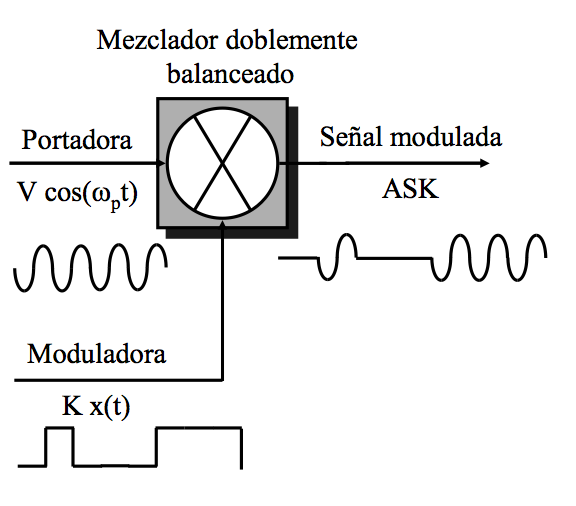
\includegraphics[scale=1, width=.3\textwidth]{ask}
    \caption{Esquema de una posible modulaci\'on ASK}
    \label{fig:ask}
\end{figure}
\paragraph{}
